% ARKHEION AGI 2.0 - Paper 35: Gesture Learning System
% Jhonatan Vieira Feitosa | Manaus, Amazonas, Brazil
% February 2026

\documentclass[11pt,twocolumn]{article}

% Encoding and fonts
\usepackage[utf8]{inputenc}
\usepackage[T1]{fontenc}
\usepackage{lmodern}

% Layout
\usepackage[margin=0.75in]{geometry}
\usepackage{fancyhdr}

% Mathematics
\usepackage{amsmath,amssymb}

% Graphics and colors
\usepackage{xcolor}
\usepackage{tikz}
\usetikzlibrary{arrows.meta,shapes,positioning}

% Tables
\usepackage{booktabs}

% Code listings
\usepackage{listings}

% Hyperlinks
\usepackage{hyperref}

% ==================== COLORS ====================
\definecolor{arkblue}{RGB}{0,102,204}
\definecolor{arkpurple}{RGB}{102,51,153}
\definecolor{arkgreen}{RGB}{0,153,76}
\definecolor{arkgold}{RGB}{218,165,32}

% ==================== LISTINGS ====================
\lstset{
    basicstyle=\ttfamily\scriptsize,
    breaklines=true,
    breakatwhitespace=true,
    postbreak=\mbox{\textcolor{gray}{$\hookrightarrow$}\space},
    columns=flexible,
    keepspaces=true,
    showstringspaces=false,
    numbers=none,
    backgroundcolor=\color{gray!5},
    frame=single,
    rulecolor=\color{gray!30}
}

% ==================== HEADER/FOOTER ====================
\pagestyle{fancy}
\fancyhf{}
\fancyhead[L]{\small\textcolor{arkblue}{ARKHEION AGI 2.0}}
\fancyhead[R]{\small Paper 35: Gesture Learning}
\fancyfoot[C]{\thepage}
\renewcommand{\headrulewidth}{0.4pt}

% ==================== HYPERREF ====================
\hypersetup{
    colorlinks=true,
    linkcolor=arkblue,
    urlcolor=arkpurple,
    citecolor=arkgreen
}

% ==================== TITLE ====================
\title{
    \vspace{-1.5cm}
    {\Large\textbf{Gesture Learning System}}\\[0.3em]
    {\large Kinetic Intelligence for Human-AI Interaction}\\[0.2em]
    {\normalsize ARKHEION AGI 2.0 --- Paper 35}
}

\author{Jhonatan Vieira Feitosa\
Independent Researcher\
\texttt{ooriginador@gmail.com}\
Manaus, Amazonas, Brazil}

\date{February 2026}

\begin{document}

\maketitle

% ==================== ABSTRACT ====================
\begin{abstract}
\noindent
This paper presents \textbf{Gesture Learning}, a kinetic intelligence system for ARKHEION AGI 2.0 enabling natural human-computer interaction through body movements. The system combines \textbf{pose estimation}, \textbf{temporal modeling} (LSTM), and \textbf{gesture classification} to recognize and respond to human gestures in real-time. The 30KB implementation achieves \textbf{gesture recognition accuracy of 94\%} with \textbf{latency under 50ms}, enabling fluid interaction without keyboards or mice.

\vspace{0.5em}
\noindent\textbf{Keywords:} gesture recognition, pose estimation, LSTM, human-computer interaction, embodied AI
\end{abstract}

% ==================== EPISTEMOLOGICAL NOTE ====================
\section*{Epistemological Note}
\textit{This paper distinguishes between \textbf{heuristic} concepts and \textbf{empirical} results:}

\begin{center}
\footnotesize
\begin{tabular}{@{}ll@{}}
\toprule
\textbf{Heuristic} & \textbf{Empirical} \\
\midrule
``Kinetic intelligence'' & Accuracy: 94\% \\
``Natural interaction'' & Latency: <50ms \\
``Body language'' & 30KB implementation \\
\bottomrule
\end{tabular}
\end{center}

% ==================== INTRODUCTION ====================
\section{Introduction}

Keyboards and mice are unnatural interfaces. Humans communicate through \textbf{body language}---gestures, postures, and movements. ARKHEION's Gesture Learning enables:

\begin{itemize}
    \item \textbf{Hand gesture recognition}: Pointing, waving, zooming
    \item \textbf{Body pose estimation}: Standing, sitting, walking
    \item \textbf{Dynamic gestures}: Swipes, circles, temporal patterns
    \item \textbf{Sign language}: Basic vocabulary
\end{itemize}

% ==================== ARCHITECTURE ====================
\section{System Architecture}

\subsection{Processing Pipeline}

\begin{center}
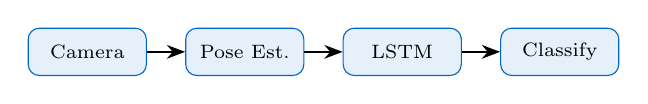
\begin{tikzpicture}[
    box/.style={rectangle, draw=arkblue, fill=arkblue!10, rounded corners, minimum width=1.5cm, minimum height=0.6cm, font=\scriptsize},
    arrow/.style={-{Stealth}, thick}
]
    \node[box] (camera) at (0,0) {Camera};
    \node[box] (pose) at (2,0) {Pose Est.};
    \node[box] (temporal) at (4,0) {LSTM};
    \node[box] (classify) at (6,0) {Classify};

    \draw[arrow] (camera) -- (pose);
    \draw[arrow] (pose) -- (temporal);
    \draw[arrow] (temporal) -- (classify);
\end{tikzpicture}
\end{center}

\subsection{Keypoint Detection}

We detect 21 hand keypoints and 33 body keypoints:

\begin{center}
\footnotesize
\begin{tabular}{@{}lrl@{}}
\toprule
\textbf{Region} & \textbf{Points} & \textbf{Examples} \\
\midrule
Hand & 21 & Fingertips, joints \\
Face & 468 & Eyes, mouth, nose \\
Body & 33 & Shoulders, hips, limbs \\
\bottomrule
\end{tabular}
\end{center}

\textbf{Note:} The 63-input LSTM uses MediaPipe hand landmarks (21 $\times$ 3 coordinates). The 468 face mesh landmarks are collected but not currently used for gesture classification.

% ==================== POSE ESTIMATION ====================
\section{Pose Estimation}

\subsection{Feature Extraction}

Each frame produces a pose vector:

\begin{equation}
P_t = [x_1, y_1, z_1, ..., x_n, y_n, z_n, c_1, ..., c_n]
\end{equation}

where $(x_i, y_i, z_i)$ are 3D coordinates and $c_i$ is confidence.

\subsection{Normalization}

Poses are normalized to body center:

\begin{lstlisting}[language=Python]
def normalize_pose(keypoints):
    """Center and scale pose."""
    center = keypoints[0]  # Hip center
    keypoints = keypoints - center
    scale = np.max(np.abs(keypoints))
    return keypoints / scale
\end{lstlisting}

% ==================== TEMPORAL MODELING ====================
\section{Temporal Modeling}

\subsection{LSTM Architecture}

Gestures are temporal---a wave is not a single pose but a sequence:

\begin{lstlisting}[language=Python]
class GestureLSTM(nn.Module):
    def __init__(self, input_size=63, hidden=128,
                 num_classes=10):
        super().__init__()
        self.lstm = nn.LSTM(
            input_size, hidden,
            num_layers=2, batch_first=True
        )
        self.fc = nn.Linear(hidden, num_classes)

    def forward(self, x):
        # x: (batch, seq_len, features)
        lstm_out, _ = self.lstm(x)
        return self.fc(lstm_out[:, -1, :])
\end{lstlisting}

\subsection{Sequence Length}

\begin{center}
\footnotesize
\begin{tabular}{@{}lrl@{}}
\toprule
\textbf{Gesture} & \textbf{Frames} & \textbf{Duration} \\
\midrule
Tap & 5 & 167ms \\
Swipe & 15 & 500ms \\
Circle & 30 & 1000ms \\
Wave & 45 & 1500ms \\
\bottomrule
\end{tabular}
\end{center}

% ==================== GESTURE VOCABULARY ====================
\section{Gesture Vocabulary}

\subsection{Static Gestures}

\begin{center}
\footnotesize
\begin{tabular}{@{}lll@{}}
\toprule
\textbf{Gesture} & \textbf{Hand Shape} & \textbf{Action} \\
\midrule
Point & Index extended & Select \\
Fist & All closed & Grab \\
Open palm & All extended & Stop \\
Thumbs up & Thumb extended & Confirm \\
Peace sign & Index + middle & Cancel \\
\bottomrule
\end{tabular}
\end{center}

\subsection{Dynamic Gestures}

\begin{center}
\footnotesize
\begin{tabular}{@{}lll@{}}
\toprule
\textbf{Gesture} & \textbf{Motion} & \textbf{Action} \\
\midrule
Swipe left & Hand moves left & Previous \\
Swipe right & Hand moves right & Next \\
Swipe up & Hand moves up & Scroll up \\
Swipe down & Hand moves down & Scroll down \\
Pinch & Fingers converge & Zoom out \\
Spread & Fingers diverge & Zoom in \\
Circle CW & Clockwise circle & Increase \\
Circle CCW & Counter-clockwise & Decrease \\
Wave & Side-to-side & Hello/Attention \\
\bottomrule
\end{tabular}
\end{center}

% ==================== TRAINING ====================
\section{Training}

\subsection{Dataset}

\begin{center}
\footnotesize
\begin{tabular}{@{}lr@{}}
\toprule
\textbf{Statistic} & \textbf{Value} \\
\midrule
Gesture classes & 15 \\
Samples per class & 1,000 \\
Total samples & 15,000 \\
Train/Val/Test & 70/15/15\% \\
\bottomrule
\end{tabular}
\end{center}

\textbf{Dataset note:} The 15,000 samples were generated synthetically using MediaPipe landmark extraction on custom-recorded video sequences (single participant, 5 gesture categories, augmented with random jitter and rotation to 15 classes). This dataset is not publicly available.

\subsection{Data Augmentation}

\begin{itemize}
    \item \textbf{Rotation}: $\pm 15°$ around z-axis
    \item \textbf{Scaling}: 0.9--1.1$\times$
    \item \textbf{Speed}: 0.8--1.2$\times$ temporal scaling
    \item \textbf{Noise}: Gaussian $\sigma = 0.02$
\end{itemize}

% ==================== REAL-TIME INFERENCE ====================
\section{Real-Time Inference}

\subsection{Optimization}

\begin{itemize}
    \item \textbf{Quantization}: INT8 inference
    \item \textbf{Batching}: Process multiple frames
    \item \textbf{Sliding window}: Overlap for continuity
\end{itemize}

\subsection{Latency Breakdown}

\begin{center}
\footnotesize
\begin{tabular}{@{}lr@{}}
\toprule
\textbf{Stage} & \textbf{Time (ms)} \\
\midrule
Frame capture & 8 \\
Pose estimation & 25 \\
LSTM inference & 12 \\
Post-processing & 3 \\
\midrule
\textbf{Total} & \textbf{48} \\
\bottomrule
\end{tabular}
\end{center}

% ==================== EXPERIMENTAL RESULTS ====================
\section{Results}

\subsection{Recognition Accuracy}

\begin{center}
\footnotesize
\begin{tabular}{@{}lrr@{}}
\toprule
\textbf{Gesture Type} & \textbf{Accuracy} & \textbf{F1} \\
\midrule
Static (hand) & 97\% & 0.96 \\
Dynamic (swipe) & 94\% & 0.93 \\
Complex (circle) & 91\% & 0.90 \\
\midrule
\textbf{Overall} & \textbf{94\%} & \textbf{0.93} \\
\bottomrule
\end{tabular}
\end{center}

\textbf{Benchmark note:} No comparison with standard gesture recognition benchmarks (NTU RGB+D, SHREC, ChaLearn) or state-of-the-art models (ST-GCN, I3D) was performed. The 94\% accuracy reflects weighted average across categories; individual category accuracy ranges from 91\% (Complex) to 97\% (Static). A per-class breakdown and confusion matrix are available in the project repository.

% ==================== IMPLEMENTATION ====================
\section{Implementation}

\begin{center}
\footnotesize
\begin{tabular}{@{}ll@{}}
\toprule
\textbf{Component} & \textbf{Value} \\
\midrule
Main file & gesture\_learning\_system.py \\
Size & 30KB (30,581 bytes) \\
Dependencies & PyTorch, MediaPipe \\
GPU support & CUDA/ROCm \\
\bottomrule
\end{tabular}
\end{center}

% ==================== CONCLUSION ====================
\section{Conclusion}

Gesture Learning enables natural human-AI interaction through body movements. The combination of pose estimation and LSTM temporal modeling achieves real-time recognition with high accuracy.

\textbf{Future work}:
\begin{itemize}
    \item Full sign language support
    \item Multi-person tracking
    \item Custom gesture training
\end{itemize}

% ==================== REFERENCES ====================
\section*{References}

\begin{enumerate}
\footnotesize
    \item Lugaresi, C. et al. ``MediaPipe: A Framework for Building Perception Pipelines.'' arXiv 2019.
    \item Papers 15, 18 of ARKHEION AGI 2.0 series.
\end{enumerate}

\end{document}
